\documentclass[preprint,12pt,aps,pra,showkeys,amsmath,amssymb,superscriptaddress,floatfix]{revtex4-2}
\usepackage[T1]{fontenc}
\usepackage[utf8]{inputenc}
\usepackage{amsmath,amssymb,amsthm,mathtools,mathrsfs}
\usepackage{microtype,booktabs,enumitem}
\usepackage{xcolor,tikz,etoolbox}
\usepackage[skins,breakable]{tcolorbox}
\usepackage{needspace}
% Keep diagram geometry independent of REVTeX preprint body spacing.
\AtBeginEnvironment{tikzpicture}{\linespread{1}\selectfont}
\usetikzlibrary{arrows.meta,positioning,calc,fit,decorations.pathreplacing}
\usepackage{graphicx}
\usepackage{hyperref}

\definecolor{MMBlue}{RGB}{0,82,155}
\definecolor{MMOrange}{RGB}{200,80,0}
\tikzset{
 mmnode/.style={draw=MMBlue,rounded corners=2pt,fill=MMBlue!4,align=left,execute at begin node={\raggedright},text width=5cm,font=\fontsize{10}{12}\selectfont,inner sep=6pt},
 mmimport/.style={mmnode,draw=black!65,fill=black!4},
 mmcandidate/.style={mmnode,draw=MMOrange,dashed,fill=MMOrange!5},
 mmrejected/.style={mmnode,draw=black,densely dotted,fill=black!8},
 mmproof/.style={->,thick,MMBlue},
 mmflow/.style={->,semithick,black!70},
 mmrepair/.style={->,dashed,thick,MMOrange},
 mmcandidatearrow/.style={->,dashed,semithick,MMOrange},
 mmnote/.style={font=\scriptsize,fill=white,inner sep=2pt,align=center}}

\usepackage[section]{placeins}
\setlength{\emergencystretch}{3em}
\setlist{itemsep=3pt,topsep=4pt}
\newtheorem{theorem}{Theorem}[section]
\newtheorem{proposition}[theorem]{Proposition}
\newtheorem{lemma}[theorem]{Lemma}
\newtheorem{corollary}[theorem]{Corollary}
\theoremstyle{definition}
\newtheorem{definition}[theorem]{Definition}
\newtheorem{example}[theorem]{Example}
\theoremstyle{remark}
\newtheorem{remark}[theorem]{Remark}
% Avoid isolated statement headings and single-line paragraph fragments.
\BeforeBeginEnvironment{theorem}{\Needspace{6\baselineskip}}
\BeforeBeginEnvironment{definition}{\Needspace{5\baselineskip}}
\BeforeBeginEnvironment{proposition}{\Needspace{5\baselineskip}}
\BeforeBeginEnvironment{lemma}{\Needspace{5\baselineskip}}
\BeforeBeginEnvironment{corollary}{\Needspace{5\baselineskip}}
\clubpenalty=5000
\widowpenalty=5000
\newcommand{\R}{\mathbb R}\newcommand{\Z}{\mathbb Z}\newcommand{\N}{\mathbb N}
\newcommand{\Pa}{\operatorname{Pa}}\newcommand{\Desc}{\operatorname{Desc}}
\newcommand{\cl}{\operatorname{cl}}\newcommand{\cost}{\operatorname{cost}}
\newcommand{\status}{\operatorname{status}}
% Faculty cards: a visual rail groups the five faculties within one agent.
% The rail has no arrowhead and does not represent a proof dependency.
\newcommand{\mmfacultybadge}[1]{%
 \node[circle,draw=MMBlue,line width=1pt,fill=white,
 minimum size=7mm,inner sep=0pt,font=\sffamily\small\bfseries,text=MMBlue]
 at ([xshift=15pt,yshift=-15pt]frame.north west) {#1};}
\newcommand{\mmfacultyrail}{%
 \draw[MMBlue!80,line width=1pt]
 ([xshift=15pt,yshift=2pt]frame.north west)--
 ([xshift=15pt,yshift=-2pt]frame.south west);}
\newtcolorbox{mmfacultybox}[2]{enhanced,breakable,
 colback=MMBlue!4,colframe=MMBlue!4,boxrule=0pt,arc=3pt,
 left=39pt,right=9pt,top=4pt,bottom=4pt,
 before skip=2pt,after skip=2pt,
 fontupper=\small\linespread{1.1}\selectfont,
 overlay unbroken={\mmfacultyrail\mmfacultybadge{#1}},
 overlay first={\mmfacultyrail\mmfacultybadge{#1}},
 overlay middle={\mmfacultyrail},overlay last={\mmfacultyrail}}
\newcommand{\mmfaculty}[3]{%
 \begin{mmfacultybox}{#1}{#2}
 {\sffamily\bfseries\color{MMBlue}#2}\par\smallskip #3
 \end{mmfacultybox}}
\newcommand{\agent}[9]{%
 \Needspace{8\baselineskip}
 \subsubsection{#1}
 \noindent\textbf{Object.} #2\par
 \noindent\textbf{Role.} #3\par\smallskip
 \mmfaculty{E}{Ego}{#4}
 \mmfaculty{M}{Memory}{#5}
 \mmfaculty{I}{Intellect}{#6}
 \mmfaculty{S}{Sense}{#7}
 \mmfaculty{A}{Action}{#8}
 \smallskip\noindent #9\par}

\usepackage{longtable,array,calc}
\providecommand{\tightlist}{\setlength{\itemsep}{2pt}\setlength{\parskip}{0pt}}
\makeatletter
\def\frontmatter@abstract@produce{\par\addvspace{\frontmatter@preabstractspace}%
\begingroup\prep@absbox\unvbox\absbox\post@absbox\endgroup
\addvspace{\frontmatter@postabstractspace}}
\makeatother
\newcommand{\field}[2]{\par\smallskip\noindent\textbf{#1.} #2\par}
\setlength{\emergencystretch}{5em}
\AtBeginEnvironment{verbatim}{\small\linespread{1.0}\selectfont}


\hypersetup{colorlinks=true,linkcolor=MMBlue,urlcolor=MMBlue,pdfauthor={Dibakar Sigdel}}

\begin{document}

\title{Poincaré Duality\\[4pt]\large An End-to-End Meta-Math Walkthrough}

\author{Dibakar Sigdel}

\affiliation{Mindverse Computing LLC, Lynnwood, WA 98087, USA}

\date{October 2026}

\begin{abstract}

A complete authored walkthrough of poincaré duality, with explicit
mathematical contracts, local verification gates, and reusable exports.
The report presents the target theorem, declared imports, a dependency
graph, five-faculty node contracts, a continuous proof, a worked
example, and a hypothesis-repair audit. It is an authored mathematical
exposition, not a deployed-agent transcript or a formal proof-assistant
certificate.

\end{abstract}\maketitle\linespread{1.12}\selectfont

\noindent\textbf{AT-05 / Algebraic Topology / Report v1}

\section{Target and import contract}

\begin{theorem}

For a closed connected oriented smooth \(n\)-manifold \(M\), prove cap
product with its integral fundamental class gives an isomorphism
\(H^k(M;\mathbb Z)\to H_{n-k}(M;\mathbb Z)\) for \(0\le k\le n\).

\end{theorem}

\subsection{Foundations and permitted imports}

Use a finite smooth triangulationK of the closed oriented manifold,
compatible orientations on top simplices, and its barycentric
subdivision. Import simplicial/cellular-to-singular homology and
cohomology comparison and subdivision invariance. In a triangulated
manifold the closed star of each simplex is contractible, and
barycentric dual blocks form a cell decomposition: the link is a sphere
and coning its subdivided chains gives the complementary-dimensional
ball. Use the chain definition of cap product with identity
\(\partial ([M]\) cap \(\alpha )=(-1)^{(k+1)}[M]\) cap \(\delta \alpha\)
for a closed fundamental cycle and a degree-k cochain, with a fixed
matching cap convention. No duality is imported; the dual differential
and identification are established below.

Use a compatible smooth (hence combinatorial) triangulation, so links
have the required sphere structure. The singular-chain filling in a
closed star is provided by a contraction of that star, not by a claim
that an arbitrary contractible space is literally a geometric cone.

\clearpage\section{Node interaction workflow}

\begin{center}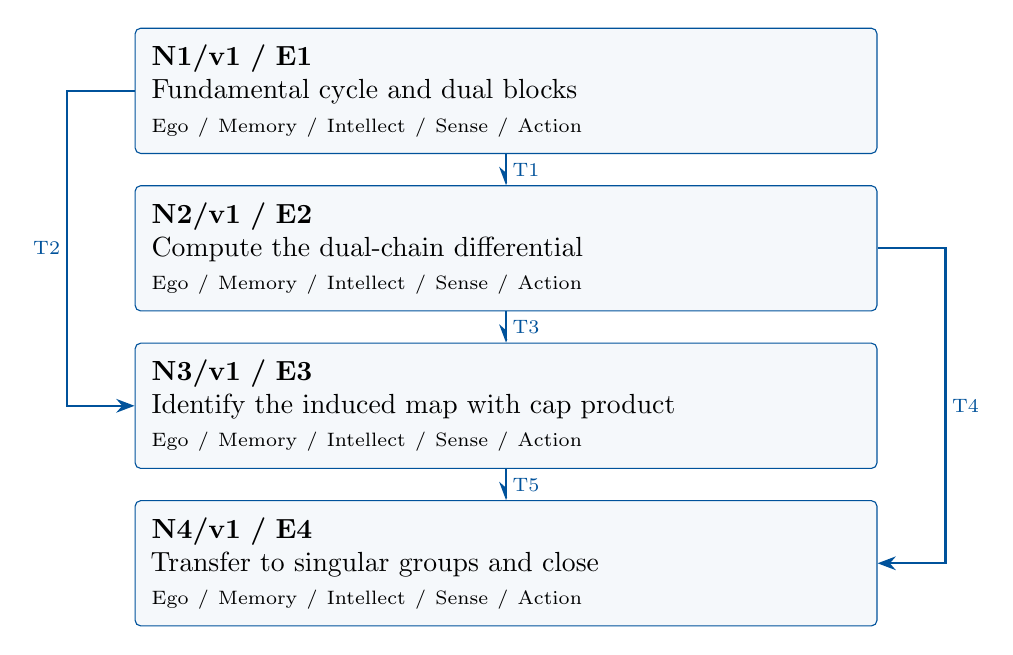
\begin{tikzpicture}[>=Stealth,x=1cm,y=1cm]

\node[mmnode,text width=9cm,minimum height=1.25cm] (N1) at (0,0.0) {\textbf{N1/v1 / E1}\\Fundamental cycle and dual blocks\\{\scriptsize Ego / Memory / Intellect / Sense / Action}};

\node[mmnode,text width=9cm,minimum height=1.25cm] (N2) at (0,-2.0) {\textbf{N2/v1 / E2}\\Compute the dual-chain differential\\{\scriptsize Ego / Memory / Intellect / Sense / Action}};

\node[mmnode,text width=9cm,minimum height=1.25cm] (N3) at (0,-4.0) {\textbf{N3/v1 / E3}\\Identify the induced map with cap product\\{\scriptsize Ego / Memory / Intellect / Sense / Action}};

\node[mmnode,text width=9cm,minimum height=1.25cm] (N4) at (0,-6.0) {\textbf{N4/v1 / E4}\\Transfer to singular groups and close\\{\scriptsize Ego / Memory / Intellect / Sense / Action}};

\draw[mmproof] (N1.south) -- node[mmnote,right] {T1} (N2.north);

\draw[mmproof] (N1.west) -- (-5.58,0) -- node[mmnote,left] {T2} (-5.58,-4) -- (N3.west);

\draw[mmproof] (N2.south) -- node[mmnote,right] {T3} (N3.north);

\draw[mmproof] (N2.east) -- (5.58,-2) -- node[mmnote,right] {T4} (5.58,-6) -- (N4.east);

\draw[mmproof] (N3.south) -- node[mmnote,right] {T5} (N4.north);

\end{tikzpicture}\end{center}

Each box is one mathematical agent containing all five faculties. Blue
arrows carry the versioned exports listed below. The layout gives a
reading order; only drawn arrows assert dependencies. Diagnostic repair
is separate from the proof DAG.

\clearpage\subsection{Versioned evidence-transfer ledger}

\begingroup\small\linespread{1.05}\selectfont

\Needspace{5\baselineskip}\field{T1: N1/E1/v1 to N2}{The fundamental cycle and a basis pairing between simplicial cochains
and dual cellular chains.}

\field{Receiving activity}{N2: Compute the dual-chain differential}

\field{Compatibility}{Use the same mathematical objects and hypotheses as the source export.
Receiving contract: Oriented dual blocks and incidence
\(numbers[\tau :\sigma ]\); prior exports E1/v1}

\Needspace{5\baselineskip}\field{T2: N1/E1/v1 to N3}{The fundamental cycle and a basis pairing between simplicial cochains
and dual cellular chains.}

\field{Receiving activity}{N3: Identify the induced map with cap product}

\field{Compatibility}{Use the same mathematical objects and hypotheses as the source export.
Receiving contract: Dual map D and cap map againstc; prior exports
E1/v1, E2/v1}

\Needspace{5\baselineskip}\field{T3: N2/E2/v1 to N3}{A degree-reversing chain identification inducing
\(H^k(K\);\(Z)\cong H_{n-k}(dualK\);Z).}

\field{Receiving activity}{N3: Identify the induced map with cap product}

\field{Compatibility}{Use the same mathematical objects and hypotheses as the source export.
Receiving contract: Dual map D and cap map againstc; prior exports
E1/v1, E2/v1}

\Needspace{5\baselineskip}\field{T4: N2/E2/v1 to N4}{A degree-reversing chain identification inducing
\(H^k(K\);\(Z)\cong H_{n-k}(dualK\);Z).}

\field{Receiving activity}{N4: Transfer to singular groups and close}

\field{Compatibility}{Use the same mathematical objects and hypotheses as the source export.
Receiving contract: Chain identification and cap comparison; prior
exports E2/v1, E3/v1}

\Needspace{5\baselineskip}\field{T5: N3/E3/v1 to N4}{The dual-cell isomorphism is the cap-product map {[}M{]} \(cap(-)\).}

\field{Receiving activity}{N4: Transfer to singular groups and close}

\field{Compatibility}{Use the same mathematical objects and hypotheses as the source export.
Receiving contract: Chain identification and cap comparison; prior
exports E2/v1, E3/v1}

\endgroup

\clearpage\section{Agent roles and five-faculty activities}\begingroup\small\linespread{1.05}\selectfont\setlist{itemsep=1pt,topsep=2pt}

\subsection{N1/v1: Fundamental cycle and dual blocks}

\field{Object and role}{Pair an oriented simplex with its transverse dual block.}

\field{Inputs}{Oriented triangulation of a closedn-manifold; foundational imports
stated in §1}

\mmfaculty{E}{Ego}{Own E1/v1: The fundamental cycle and a basis pairing between simplicial
cochains and dual cellular chains.}

\mmfaculty{M}{Memory}{Retain Oriented triangulation of a closedn-manifold; foundational
imports stated in §1; keep their assumptions and versions attached.}

\mmfaculty{I}{Intellect}{Pair an oriented simplex with its transverse dual block.}

\mmfaculty{S}{Sense}{Closedness cancels all faces; orientability makes their signs globally
compatible.}

\mmfaculty{A}{Action}{Carry out the numbered deductions and publish E1/v1 together with its
hypotheses and proof location.}

\smallskip\noindent\textbf{Numbered mathematical activities}

\begin{enumerate}[label=N1.\arabic*,leftmargin=3.4em]

\item Letc be the sum of compatibly orientedn-simplices.

\item Every \((n-1)\)-face is shared twice with opposite induced signs, so
\(\partial c=0\).

\item Its local coefficient at every oriented manifold point is+1, so it
represents the integral fundamental class{[}M{]}.

\item For an orientedk-simplex \(\sigma\), its dual blockD \(\sigma\) is the
union of barycentric flags beginning at \(\sigma\) and continuing
through cofaces up to top-dimensional simplices.

\item It has dimension \(n-k\).

\item OrientD \(\sigma\) so the ordered orientation of \(\sigma\) followed by
its transverse dual orientation gives the orientation of M.

\item These blocks bijectively pair k-simplices with \((n-k)\)-cells.

\end{enumerate}

\field{Export E1/v1}{The fundamental cycle and a basis pairing between simplicial cochains
and dual cellular chains.}

\field{Acceptance gate}{Closedness cancels all faces; orientability makes their signs globally
compatible. Publish only after checking every displayed deduction.}

\field{Targeted repair}{If the check fails, revise N1: Closedness cancels all faces;
orientability makes their signs globally compatible. Recheck dependent
nodes N2, N3, N4.}

\clearpage

\subsection{N2/v1: Compute the dual-chain differential}

\field{Object and role}{Compare boundary flags for \(\sigma\) and its immediate cofaces.}

\field{Inputs}{Oriented dual blocks and incidence \(numbers[\tau :\sigma ]\); prior
exports E1/v1}

\mmfaculty{E}{Ego}{Own E2/v1: A degree-reversing chain identification inducing
\(H^k(K\);\(Z)\cong H_{n-k}(dualK\);Z).}

\mmfaculty{M}{Memory}{Retain Oriented dual blocks and incidence \(numbers[\tau :\sigma ]\);
prior exports E1/v1; keep their assumptions and versions attached.}

\mmfaculty{I}{Intellect}{Compare boundary flags for \(\sigma\) and its immediate cofaces.}

\mmfaculty{S}{Sense}{Ignoring signs would only justify a mod 2 statement, not integral
duality.}

\mmfaculty{A}{Action}{Carry out the numbered deductions and publish E2/v1 together with its
hypotheses and proof location.}

\smallskip\noindent\textbf{Numbered mathematical activities}

\begin{enumerate}[label=N2.\arabic*,leftmargin=3.4em]

\item The codimension-one boundary faces of \(D\sigma\) correspond to
(k+1)-cofaces \(\tau\) of \(\sigma\) and are copies of \(D\tau\).

\item Other flag faces occur twice with opposite subdivision signs and cancel.

\item \(If[\tau :\sigma ]\) is the signed simplex incidence, moving the
normal-to-\(\sigma\) direction across itsk tangent directions and using
outward-first boundary orientation gives the coefficient
\((-1)^{(k+1)}[\tau :\sigma ]\).

\item Thus
\(\partial D\sigma =(-1)^{(k+1)}\sum _{\tau \supset \sigma }[\tau :\sigma ]D\tau\).

\item For the cochain basis \(\sigma *\),
\(\delta \sigma *=\sum [\tau :\sigma ]\tau *\).

\item Hence the degree-reversing basis map D satisfies
\(\partial D\alpha =(-1)^{(k+1)}D\delta \alpha\).

\item It sends cocycles to cycles and coboundaries to boundaries, with an
inverse on bases and the same differential relation.

\end{enumerate}

\field{Export E2/v1}{A degree-reversing chain identification inducing
\(H^k(K\);\(Z)\cong H_{n-k}(dualK\);Z).}

\field{Acceptance gate}{Ignoring signs would only justify a mod 2 statement, not integral
duality. Publish only after checking every displayed deduction.}

\field{Targeted repair}{If the check fails, revise N2: Ignoring signs would only justify a mod 2
statement, not integral duality. Recheck dependent nodes N3, N4.}

\clearpage

\begingroup\footnotesize\linespread{1.05}\selectfont\let\small\footnotesize

\subsection{N3/v1: Identify the induced map with cap product}

\field{Object and role}{Use local carriers to compare two chain constructions, not only abstract
ranks.}

\field{Inputs}{Dual map D and cap map againstc; prior exports E1/v1, E2/v1}

\mmfaculty{E}{Ego}{Identify cap product with the dual-cell isomorphism.}

\mmfaculty{M}{Memory}{Import E1/v1, E2/v1, the cap-chain formula, and contractible closed
stars.}

\mmfaculty{I}{Intellect}{Use local carriers to compare two chain constructions, not only abstract
ranks.}

\mmfaculty{S}{Sense}{An abstract group isomorphism would not identify the specified canonical
map.}

\mmfaculty{A}{Action}{Build the carrier homotopy and publish E3/v1.}

\smallskip\noindent\textbf{Numbered mathematical activities}

\begin{enumerate}[label=N3.\arabic*,leftmargin=3.4em]

\item View the reversed cochain complex as a chain complex with degree
\(r=n-k\) and differential \((-1)^{(k+1)}\delta\).

\item After mapping dual cellular chains to singular chains in the
subdivision, both D and \(C:\alpha \mapsto c\) cap \(\alpha\) are chain
maps to singular chains.

\item For a basis \(\sigma *\) both images are supported in the closed star of
\(\sigma\): dual flags lie there, and every cap term comes from a top
simplex containing \(\sigma\).

\item The carrier is nested under the differential since cofaces have stars
contained in that of \(\sigma\).

\item In degree 0, for a top-simplex cochain, the dual barycenter and
cap-selected vertex have the same oriented augmentation.

\item Construct a chain homotopy upward on this free basis: if H is already
defined one degree lower, \(z=(D-C)(\sigma *)-H(d\sigma *)\) is a cycle
in star \(\sigma\), with zero augmentation when it is a0-cycle.

\item The star is contractible, so this cycle bounds; use the induced
singular-chain contraction to choose a filling \(H(\sigma^*)\).

\item Inductively \(D-C=\partial H+Hd\).

\item Thus the two maps induce the same map on homology.

\item This is the explicit local-carrier comparison between dual blocks and
the cap construction.

\end{enumerate}

\field{Export E3/v1}{The dual-cell isomorphism is the cap-product map {[}M{]} \(cap(-)\).}

\field{Acceptance gate}{Identify the canonical cap-product map, not merely isomorphic groups.}

\field{Targeted repair}{Rebuild the carrier homotopy, then recheck N4.}

\endgroup

\clearpage

\subsection{N4/v1: Transfer to singular groups and close}

\field{Object and role}{Apply the imported comparison maps compatibly.}

\field{Inputs}{Chain identification and cap comparison; prior exports E2/v1, E3/v1}

\mmfaculty{E}{Ego}{Own E4/v1: Integral Poincaré duality with the specified
fundamental-class cap map.}

\mmfaculty{M}{Memory}{Retain Chain identification and cap comparison; prior exports E2/v1,
E3/v1; keep their assumptions and versions attached.}

\mmfaculty{I}{Intellect}{Apply the imported comparison maps compatibly.}

\mmfaculty{S}{Sense}{The theorem is for closed oriented manifolds; boundary and
nonorientability change the target coefficients or relative groups.}

\mmfaculty{A}{Action}{Carry out the numbered deductions and publish E4/v1 together with its
hypotheses and proof location.}

\smallskip\noindent\textbf{Numbered mathematical activities}

\begin{enumerate}[label=N4.\arabic*,leftmargin=3.4em]

\item Simplicial cohomology of K and cellular homology of its dual
decomposition identify with the respective singular groups of M.

\item These comparison maps commute with subdivision and cap products by the
chain constructions used in node3.

\item Since D is an isomorphism on the reversed complexes, it is an
isomorphism on their homology.

\item Since C induces the same map, cap product with{[}M{]} gives
\(H^k(M\);\(Z)\to H_{n-k}(M\);Z) as an isomorphism for every
\(0\le k\le n\).

\item Reversing orientation negates{[}M{]} and the resulting map but preserves
its invertibility.

\end{enumerate}

\field{Export E4/v1}{Integral Poincaré duality with the specified fundamental-class cap map.}

\field{Acceptance gate}{The theorem is for closed oriented manifolds; boundary and
nonorientability change the target coefficients or relative groups.
Publish only after checking every displayed deduction.}

\field{Targeted repair}{If the check fails, revise N4: The theorem is for closed oriented
manifolds; boundary and nonorientability change the target coefficients
or relative groups. Withhold this terminal result until its gate passes.}

\endgroup\clearpage\section{Continuous mathematical proof}\label{sec:proof}

Read these steps in order as one proof; the diagram is optional.
Numbered activities identify the specific constructions and deductions
owned by each node.

\subsection{§4.N1 --- Fundamental cycle and dual
blocks}\label{n1-fundamental-cycle-and-dual-blocks}

\begin{enumerate}
\def\labelenumi{\arabic{enumi}.}
\item
  Letc be the sum of compatibly orientedn-simplices.
\item
  Every \((n-1)\)-face is shared twice with opposite induced signs, so
  \(\partial c=0\).
\item
  Its local coefficient at every oriented manifold point is+1, so it
  represents the integral fundamental class{[}M{]}.
\item
  For an orientedk-simplex \(\sigma\), its dual blockD \(\sigma\) is the
  union of barycentric flags beginning at \(\sigma\) and continuing
  through cofaces up to top-dimensional simplices.
\item
  It has dimension \(n-k\).
\item
  OrientD \(\sigma\) so the ordered orientation of \(\sigma\) followed
  by its transverse dual orientation gives the orientation of M.
\item
  These blocks bijectively pair k-simplices with \((n-k)\)-cells.
\end{enumerate}

\subsection{§4.N2 --- Compute the dual-chain
differential}\label{n2-compute-the-dual-chain-differential}

\begin{enumerate}
\def\labelenumi{\arabic{enumi}.}
\item
  The codimension-one boundary faces of \(D\sigma\) correspond to
  (k+1)-cofaces \(\tau\) of \(\sigma\) and are copies of \(D\tau\).
\item
  Other flag faces occur twice with opposite subdivision signs and
  cancel.
\item
  \(If[\tau :\sigma ]\) is the signed simplex incidence, moving the
  normal-to-\(\sigma\) direction across itsk tangent directions and
  using outward-first boundary orientation gives the coefficient
  \((-1)^{(k+1)}[\tau :\sigma ]\).
\item
  Thus
  \(\partial D\sigma =(-1)^{(k+1)}\sum _{\tau \supset \sigma }[\tau :\sigma ]D\tau\).
\item
  For the cochain basis \(\sigma *\),
  \(\delta \sigma *=\sum [\tau :\sigma ]\tau *\).
\item
  Hence the degree-reversing basis map D satisfies
  \(\partial D\alpha =(-1)^{(k+1)}D\delta \alpha\).
\item
  It sends cocycles to cycles and coboundaries to boundaries, with an
  inverse on bases and the same differential relation.
\end{enumerate}

\subsection{§4.N3 --- Identify the induced map with cap
product}\label{n3-identify-the-induced-map-with-cap-product}

\begin{enumerate}
\def\labelenumi{\arabic{enumi}.}
\item
  View the reversed cochain complex as a chain complex with degree
  \(r=n-k\) and differential \((-1)^{(k+1)}\delta\).
\item
  After mapping dual cellular chains to singular chains in the
  subdivision, both D and \(C:\alpha \mapsto c\) cap \(\alpha\) are
  chain maps to singular chains.
\item
  For a basis \(\sigma *\) both images are supported in the closed star
  of \(\sigma\): dual flags lie there, and every cap term comes from a
  top simplex containing \(\sigma\).
\item
  The carrier is nested under the differential since cofaces have stars
  contained in that of \(\sigma\).
\item
  In degree 0, for a top-simplex cochain, the dual barycenter and
  cap-selected vertex have the same oriented augmentation.
\item
  Construct a chain homotopy upward on this free basis: if H is already
  defined one degree lower, \(z=(D-C)(\sigma *)-H(d\sigma *)\) is a
  cycle in star \(\sigma\), with zero augmentation when it is a0-cycle.
\item
  The star is contractible, so this cycle bounds; use the induced
  singular-chain contraction to choose a filling \(H(\sigma^*)\).
\item
  Inductively \(D-C=\partial H+Hd\).
\item
  Thus the two maps induce the same map on homology.
\item
  This is the explicit local-carrier comparison between dual blocks and
  the cap construction.
\end{enumerate}

\subsection{§4.N4 --- Transfer to singular groups and
close}\label{n4-transfer-to-singular-groups-and-close}

\begin{enumerate}
\def\labelenumi{\arabic{enumi}.}
\item
  Simplicial cohomology of K and cellular homology of its dual
  decomposition identify with the respective singular groups of M.
\item
  These comparison maps commute with subdivision and cap products by the
  chain constructions used in node3.
\item
  Since D is an isomorphism on the reversed complexes, it is an
  isomorphism on their homology.
\item
  Since C induces the same map, cap product with{[}M{]} gives
  \(H^k(M\);\(Z)\to H_{n-k}(M\);Z) as an isomorphism for every
  \(0\le k\le n\).
\item
  Reversing orientation negates{[}M{]} and the resulting map but
  preserves its invertibility.
\end{enumerate}

\hfill$\square$

\section{Worked orchestration}

On an oriented torus, \(H^{0}=Z\) pairs with the fundamental2-cycle,
\(H^{2}=Z\) pairs with a point class, and \(H^{1}=Z^{2}\) pairs with the
two complementary1-cycle directions. Using product orientation, the
degree 1 classes are exchanged with complementary cycles up to the cap
convention's signs. The dual-block proof supplies the isomorphism rather
than only comparing these ranks.

\subsection{Boundary and hypothesis audit}

For a disk, \(H^{0}(D^{2}\);\(Z)=Z\) but \(H_{2}(D^{2}\);\(Z)=0\), so
the absolute closed-manifold formula fails. For a nonorientable closed
manifold an untwisted integral fundamental class need not exist. Sense
blocks the initial fundamental-cycle gate; relative or local-coefficient
duality is a distinct theorem.

\section{Illustrative failure and repair}

The following is an authored diagnostic scenario. Changed assumptions
define a new contract; they do not retroactively prove the original
statement.

\subsection{Failure and correction}
This is an authored teaching trace, not a recorded agent run.

\begin{enumerate}
\def\labelenumi{\arabic{enumi}.}
\tightlist
\item
  \textbf{Ego \(\to\) Memory:} register the §1 theorem, imports, and
  requested exports before beginning the proof.
\item
  \textbf{Intellect \(\to\) Action:} choose the bridges in §3 and carry
  out the numbered activities in §4; transmit only established E-exports
  along the §2 DAG.
\item
  \textbf{Sense \(\to\) responsible node:} test the specific
  boundary/failure in §5 and the node's individual audit. A failing
  candidate is withheld; downstream nodes may not use it.
\item
  \textbf{Memory + Intellect:} identify whether the error is an omitted
  condition, an invalid inference, or an attempted extension beyond the
  theorem. Restore the exact contract or explicitly state a different
  one.
\item
  \textbf{Action:} redo the affected mathematical activity using the
  repaired condition or inference. Recheck consuming nodes, rather than
  feeding their conclusions back as premises.
\item
  \textbf{Ego:} publish only the supported export with its assumptions
  and proof location. A hypothetical revised export is v2; the written
  proof here is the v1 exposition, not a claim that this repair was
  executed.
\end{enumerate}

\subsection{Hypothesis boundary}
For a disk, \(H^{0}(D^{2}\);\(Z)=Z\) but \(H_{2}(D^{2}\);\(Z)=0\), so
the absolute closed-manifold formula fails. For a nonorientable closed
manifold an untwisted integral fundamental class need not exist. Sense
blocks the initial fundamental-cycle gate; relative or local-coefficient
duality is a distinct theorem.

\subsection{Version and recheck}
Treat any changed assumption as a new contract. Recheck the revised
export and all of its descendants. A backward diagnostic never
establishes an earlier theorem. This is an authored teaching trace, not
an execution log.

\par\medskip\begingroup\small\linespread{1.0}\selectfont\noindent\textbf{Provenance.} This authored proof is complete relative to its declared imports. Reuse
each export with its assumptions, proof, and version. The original
Markdown remains available for comparison.
\par\endgroup

\par\smallskip\begingroup\small\linespread{1.0}\selectfont\noindent\textbf{Further reading.} \begin{itemize}
\tightlist
\item
  \href{https://pi.math.cornell.edu/~hatcher/AT/AT.pdf}{Allen Hatcher,
  Algebraic Topology: covering spaces, cellular homology, and cap
  products}.
\end{itemize}\par\endgroup

\end{document}
